
\subsection{Hierarchy}


\begin{frame}[c]{Why Hierarchy?}
    \Large
    \pause
    If there is a connection cost, hierarchies are more efficient \cite{mengistu2016evolutionary}. 
    
    \pause
    Especially when tasks change regularly.
\end{frame}


\begin{frame}[c]{Why Hierarchy? II}
    \Large
    \begin{itemize}[<+(1)->]
        \item Reduced Training Time
        \item Reduced Memory Usage
        \item Learned patterns are recombined at higher levels
    \end{itemize}
\end{frame}


\begin{frame}[c]{What Hierarchy}
    \pause
                                        % trim = left bottom right top
    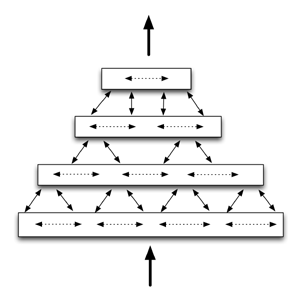
\includegraphics[width=\textwidth, trim = 0 55 0 60, clip]{hierarchy}
\end{frame}


\begin{frame}[c]{For What}
    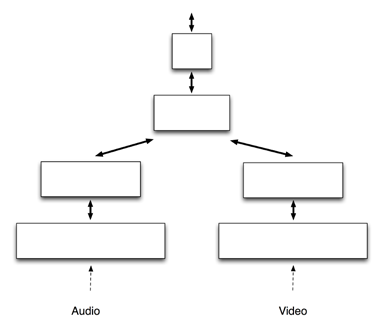
\includegraphics[height=0.9\textheight]{hierarchy_2} 
\end{frame}


\subsection{Regions}

\begin{frame}[c]{Introduction - Region}
    \pause
                                        % trim = left bottom right top
    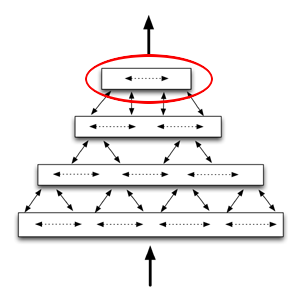
\includegraphics[width=\textwidth, trim = 0 55 0 54, clip]{region}
\end{frame}




